\documentclass{standalone}
\usepackage{tikz}
\begin{document}
    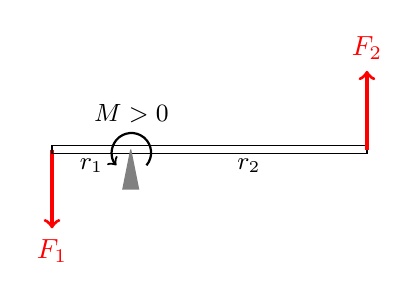
\begin{tikzpicture}
      % kraftar
      \draw [very thick, ->,red] (0,0) -- (0,-1) node [below] {$F_1$};
      \draw [] (0,-0.05) rectangle (4,0.05);
      \draw [color=gray, fill=gray] (1,0)--(1.1,-0.5)--(0.9,-0.5) -- (1,0);
      \draw [very thick, ->,red] (4,0) -- (4,1) node [above] {$F_2$};
      %merkingar
      \draw [thick,->] (1.2,-0.2) arc (-40:220:0.25) node [midway,above] {\small $M>0$};
      %\fill (1,0) circle (1pt);
      %\draw (1,0) node[above]{\small A};
      \draw (0.5,-0.2) node[]{\small $r_1$};
      \draw (2.5,-0.2) node[]{\small $r_2$};
    \end{tikzpicture}
\end{document}
